% boston_20260828_v2.tex
% Regional Special Sessions — Building Strong Health Systems for the Future
% Harvard T.H. Chan School of Public Health / Roche · Hilton Boston Back Bay
% Viernes 28 de agosto de 2026, 8:30–9:30 · Track América Latina
% Build instruction: 20260826_COMUNIDAD_BUILDINST_boston_deck_v2 (Debb)
%
% v2 — cambios respecto a v1:
%   (1) Paleta de cuatro elementos: azul de estructura, cálido SOLO para cifras,
%       banda gris tenue, regla bajo el título.
%   (2) Cuatro elementos visuales nuevos (Fig. 1-4) además de la gráfica ONU.
%   (3) Lenguaje reescrito: se elimina la antítesis repetida, las frases
%       destacadas bajan de diez a cuatro, los fragmentos pasan a oraciones.
%   (4) Aparato de fuentes movido a dos láminas finales (resuelve el desborde
%       de 19.17pt en la antigua lámina 15).
%   (5) La antigua lámina 22 se divide en dos: "quiénes" e "independencia".
%       El deck queda en 26 láminas de contenido + 2 de fuentes.
%
% RESUELTO POR CLAUDE CODE, 2026-08-26 (instrucciones v2, Tareas A–C):
%   - Argentina: sin registros en CEPALSTAT 3136 (aporta) ni 3138 (afiliada),
%     ningún año. Gráfica con siete barras y nota activada (Tarea A, regla del hueco declarado).
%   - Imagen ONU: wpp2024_lac_broad_age_groups.png, oficial LAC (eje a 400 M), pie incrustado.
%   - Figuras 1 y 2 cotejadas contra verificaciones_boston_v1.md: sin discrepancias.
% Compilar en Overleaf con pdfLaTeX (dos pasadas); ver verificaciones_boston_v2.md.
%
% Restricción dura: cero ecuaciones, cero notación matemática, cero letras griegas.

\documentclass[aspectratio=169,11pt]{beamer}

\usepackage[utf8]{inputenc}
\usepackage[T1]{fontenc}
\usepackage[spanish,es-noshorthands]{babel}
\usepackage[scaled=0.95]{helvet}
\usepackage{graphicx}
\usepackage{booktabs}
\usepackage{colortbl}
\usepackage{xcolor}
\usepackage{tikz}
\usepackage{pgfplots}
\pgfplotsset{compat=1.18}
\usetikzlibrary{arrows.meta}

\usetheme{default}
\usecolortheme{default}
\usefonttheme{professionalfonts}

\setbeamertemplate{navigation symbols}{}
\setbeamertemplate{footline}[frame number]
\setbeamertemplate{itemize items}{--}
\setbeamertemplate{blocks}[default]

%========================================================================
% PALETA — cuatro elementos, ninguno más
%========================================================================
\definecolor{acento}{RGB}{24,54,92}      % azul de estructura
\definecolor{dato}{RGB}{176,84,28}       % cálido: EXCLUSIVO para cifras
\definecolor{banda}{RGB}{238,241,246}    % gris tenue: tablas y transiciones
\definecolor{grisfino}{RGB}{120,120,120} % pies de fuente

\setbeamercolor{title}{fg=acento}
\setbeamercolor{frametitle}{fg=acento}
\setbeamercolor{structure}{fg=acento}
\setbeamercolor{itemize item}{fg=acento}
\setbeamercolor{enumerate item}{fg=acento}
\setbeamercolor{normal text}{fg=black,bg=white}
\setbeamercolor{footline}{fg=grisfino}
\setbeamerfont{frametitle}{size=\large,series=\bfseries}
\setbeamerfont{title}{size=\Large,series=\bfseries}
\setbeamerfont{footline}{size=\scriptsize}

% Título con regla fina debajo
\setbeamertemplate{frametitle}{%
  \vspace*{0.9em}%
  {\usebeamerfont{frametitle}\usebeamercolor[fg]{frametitle}\insertframetitle}%
  \\[0.28em]%
  {\color{acento}\rule{\textwidth}{0.7pt}}%
  \vspace*{-0.2em}%
}

%========================================================================
% UTILERÍA
%========================================================================
% Cifra: el color cálido se reserva exclusivamente para datos.
\newcommand{\cifra}[1]{\textcolor{dato}{\textbf{#1}}}
% Palabra clave conceptual: azul, sin negritas de más.
\newcommand{\clave}[1]{\textcolor{acento}{\textbf{#1}}}
% Frase destacada. Se usa CUATRO veces en todo el deck. No añadir más.
\newcommand{\destacar}[1]{%
  \vspace{0.5em}%
  \begin{center}%
    \colorbox{banda}{\parbox{0.92\textwidth}{\centering\vspace{0.3em}\textbf{#1}\vspace{0.3em}}}%
  \end{center}%
}
% Cierre en prosa, sin caja y sin negritas: alternativa deliberada a \destacar.
\newcommand{\cierre}[1]{\vspace{0.5em}\par{#1}}
% Pie de fuente: UNA línea. El aparato completo va en las láminas finales.
\newcommand{\pie}[1]{\vfill{\scriptsize\textcolor{grisfino}{#1}}}
% Lámina de transición sobre banda.
\newcommand{\frase}[1]{\begin{center}\Large\textbf{\textcolor{acento}{#1}}\end{center}}

\setlength{\leftmargini}{1.2em}
\setlength{\parskip}{0pt}

\title{Demografía, espacio fiscal y una nueva seguridad social}
\subtitle{Lo que esta semana no discutió}
\author{Héctor Juan Villarreal Páez}
\institute{ITED · Escuela de Gobierno y Transformación Pública · Tecnológico de Monterrey\\[0.4em]
Comunidad Latinoamericana del Conocimiento sobre Financiamiento de la Salud}
\date{Regional Special Sessions · \emph{Building Strong Health Systems for the Future}\\Boston, 28 de agosto de 2026}

\begin{document}

%=======================================================================
% APERTURA
%=======================================================================

% ---------- 1 ----------
\begin{frame}[plain]
  \titlepage
  % Logo institucional solo en portada:
  % \begin{center}\includegraphics[height=1.1cm]{logo_tec.png}\end{center}
\end{frame}

% ---------- 2 ----------
\begin{frame}{Lo que esta semana no discutió}
  \begin{itemize}
    \item Durante cuatro días revisamos compra estratégica, pago por valor, aseguramiento social y política de la reforma.
    \item Todo ese material responde a una misma pregunta: \clave{cómo gastar mejor lo que hay}.
    \item Falta otra pregunta, y de ella quiero hablar hoy: qué ocurre cuando cambia la estructura por edades de la población.
  \end{itemize}
  \cierre{Voy a plantear dos restricciones. La primera ya está determinada y no la mueve ninguna política. La segunda todavía se decide, y se decide ahora.}
\end{frame}

%=======================================================================
% MOVIMIENTO 1 — La demografía ya está decidida
%=======================================================================

% ---------- 3 ----------
\begin{frame}{América Latina y el Caribe: población por grandes grupos de edad}
  \begin{center}
    % Imagen oficial del portal WPP 2024, agregado "Latin America and the Caribbean"
    % (MD5 idéntico al archivo del sitio; eje vertical a 400 millones, NO la versión LLDC).
    % Pie de atribución incrustado (CC BY 3.0 IGO). No recortar.
    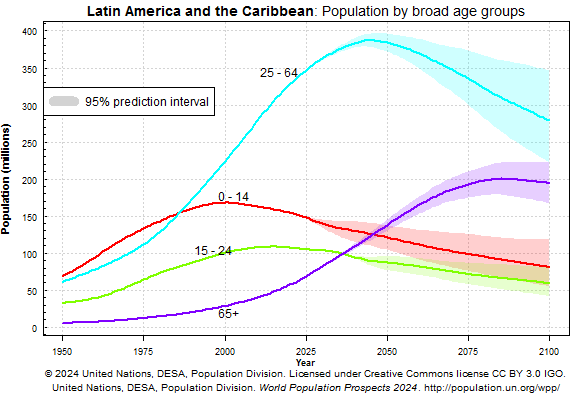
\includegraphics[height=0.78\textheight,keepaspectratio]{wpp2024_lac_broad_age_groups.png}
  \end{center}
\end{frame}

% ---------- 4 ----------
\begin{frame}{Lo que ya está contabilizado}
  \begin{itemize}
    \item Las bandas de las líneas de 65 y más y de 25 a 64 casi no se abren hasta bien entradas las décadas de 2030 y 2040.
    \item La razón es sencilla: esas personas \clave{ya nacieron}.
    \item Lo que sí es incierto es la fecundidad. La banda de 0 a 14 empieza a abrirse desde el final de esta década.
    \item Hacia \cifra{2046} habrá en la región más personas de 65 y más que niños menores de 15 años.
  \end{itemize}
  \cierre{El envejecimiento que viene no depende de lo que decidamos ahora. Ya está en los registros de nacimiento.}
  \pie{Naciones Unidas, DESA, \emph{World Population Prospects 2024}. Detalle de fuentes al final.}
\end{frame}

% ---------- 5 ----------
\begin{frame}{El envejecimiento del envejecimiento}
  \begin{itemize}
    \item La población de 80 años y más pasa de \cifra{12 millones} en 2024 a \cifra{37 millones} en 2050.
    \item Su peso sobre el total sube de 1.9\,\% a 5.1\,\%: se triplica en una generación.
    \item Es el grupo que concentra la dependencia funcional y el cuidado de largo plazo, donde el gasto deja de ser episódico y se vuelve continuo.
  \end{itemize}
  \pie{CEPAL (2025), Serie Población y Desarrollo 140. Detalle de fuentes al final.}
\end{frame}

% ---------- 6 ----------
\begin{frame}{La ventana se cierra en 2028}
  \begin{itemize}
    \item El bono demográfico regional termina, en promedio, en \cifra{2028}. Es decir, dentro de dos años.
    \item En Costa Rica, Colombia, Chile y Brasil ya terminó.
    \item Entre 2024 y 2050 la población de 65 y más pasa de \cifra{65} a \cifra{138 millones} de personas.
  \end{itemize}
  \cierre{La ventana que la región nunca aprovechó del todo se está cerrando dentro del horizonte de esta administración, no de la siguiente.}
  \pie{CEPAL (2025), Serie Población y Desarrollo 140. Detalle de fuentes al final.}
\end{frame}

%=======================================================================
% MOVIMIENTO 2 — El espacio fiscal sí es una decisión
%=======================================================================

% ---------- 7 ----------
\begin{frame}[plain]
  \vfill
  \begin{center}
    \colorbox{banda}{\parbox{0.86\textwidth}{\vspace{1.2em}\centering
      \Large\textbf{\textcolor{acento}{Lo anterior está dado.}}\\[0.5em]
      \Large\textbf{\textcolor{acento}{Lo que sigue, no.}}
      \vspace{1.2em}}}
  \end{center}
  \vfill
\end{frame}

% ---------- 8 ----------
\begin{frame}{Gasto público críticamente bajo}
  \begin{columns}[T]
    \begin{column}{0.52\textwidth}
      \small
      \begin{itemize}
        \item México destina \cifra{2.7\,\%} del PIB a salud desde el gobierno general, con la seguridad social incluida. El promedio regional es \cifra{4.1\,\%}.
        \item Lo que el Estado no paga lo pagan las familias, casi siempre por urgencia y sin haberlo previsto.
        \item En México, \cifra{41\,\%} del gasto corriente en salud sale directamente del bolsillo de los hogares. En la región, \cifra{30\,\%}.
      \end{itemize}
      \cierre{\small Es la forma más regresiva de financiar salud que existe.}
    \end{column}
    \begin{column}{0.46\textwidth}
      \vspace{0.6em}
      % ---- FIGURA 1: gasto público y gasto de bolsillo ----
      \begin{center}
      \begin{tikzpicture}[scale=0.80, transform shape]
        \begin{axis}[
          ybar, width=3.6cm, height=3.4cm,
          bar width=18pt,
          ymin=0, ymax=5.6, ytick={0,2,4},
          enlarge x limits=1.1,
          ylabel={\tiny \% del PIB},
          symbolic x coords={México,Región},
          xtick=data,
          tick label style={font=\tiny},
          label style={font=\tiny},
          nodes near coords, nodes near coords style={font=\tiny,color=black,anchor=south,xshift=7pt},
          axis lines=left, ymajorgrids, grid style={gray!20},
          title style={font=\tiny\bfseries, color=acento},
          title={Gasto público en salud}
        ]
          \addplot[fill=dato, draw=dato] coordinates {(México,2.7) (Región,4.1)};
        \end{axis}
      \end{tikzpicture}

      \vspace{0.5em}

      \begin{tikzpicture}[scale=0.80, transform shape]
        \begin{axis}[
          ybar, width=3.6cm, height=3.4cm,
          bar width=18pt,
          ymin=0, ymax=55, ytick={0,20,40},
          enlarge x limits=1.1,
          ylabel={\tiny \% del gasto},
          symbolic x coords={México,Región},
          xtick=data,
          tick label style={font=\tiny},
          label style={font=\tiny},
          nodes near coords, nodes near coords style={font=\tiny,color=black,anchor=south,xshift=7pt},
          axis lines=left, ymajorgrids, grid style={gray!20},
          title style={font=\tiny\bfseries, color=acento},
          title={Gasto de bolsillo}
        ]
          \addplot[fill=acento, draw=acento] coordinates {(México,41) (Región,30)};
        \end{axis}
      \end{tikzpicture}
      \end{center}
    \end{column}
  \end{columns}
  \pie{OMS, \emph{Global Health Expenditure Database}, 2023. Detalle de fuentes al final.}
\end{frame}

% ---------- 9 ----------
\begin{frame}{Pensiones desplazan salud}
  \begin{columns}[T]
    \begin{column}{0.55\textwidth}
      \small
      \begin{itemize}
        \item Las promesas previsionales maduraron antes de que se ampliara la base contributiva.
        \item Las pensiones no contributivas ampliaron la cobertura de manera real, y su costo fiscal crece cada año.
        \item Sin reforma paramétrica, el gasto en pensiones termina desplazando todo lo demás.
      \end{itemize}
    \end{column}
    \begin{column}{0.43\textwidth}
      \vspace{1.2em}
      % ---- FIGURA 2: esquema del espacio fiscal (SIN datos, SIN ejes) ----
      \begin{center}
      \begin{tikzpicture}[scale=0.92, transform shape]
        \draw[draw=gray!60, thick] (0,0) rectangle (6,0.85);
        \node[font=\tiny, gray] at (3,1.15) {Espacio fiscal disponible};
        \fill[dato!85] (0,0) rectangle (3.9,0.85);
        \node[font=\scriptsize\bfseries, white] at (1.95,0.42) {Pensiones};
        \fill[acento!25] (3.9,0) rectangle (6,0.85);
        \node[font=\scriptsize\bfseries, acento] at (4.95,0.42) {Salud};
        \draw[-{Latex[length=2mm]}, dato, very thick] (3.9,-0.45) -- (5.1,-0.45);
        \node[font=\tiny, dato] at (2.5,-0.45) {crece};
        \node[font=\tiny, acento] at (5.6,-0.9) {se comprime};
      \end{tikzpicture}
      \end{center}
      \vspace{0.4em}
      {\tiny\color{grisfino}Esquema conceptual, sin escala.}
    \end{column}
  \end{columns}
  \destacar{Reformar pensiones no es un tema separado de financiar salud: es su condición previa.}
\end{frame}

% ---------- 10 ----------
\begin{frame}{Un solo problema fiscal}
  \begin{itemize}
    \item Pensiones, salud y cuidados compiten por el \clave{mismo espacio presupuestario}.
    \item Conviene analizarlos como un solo sistema, y no como tres programas con presupuestos separados.
    \item Cualquier propuesta que dependa de impuestos generales tiene que demostrar que se sostiene durante veinte años, no durante un sexenio.
  \end{itemize}
\end{frame}

%=======================================================================
% MOVIMIENTO 3 — La tenaza
%=======================================================================

% ---------- 11 ----------
\begin{frame}{Dos cosas al mismo tiempo}
  \begin{itemize}
    \item Un sistema de salud tiene que lograr dos cosas a la vez.
    \item Que la gente \clave{no se arruine} cuando se enferma.
    \item Que \clave{valga la pena} estar dentro del sistema contributivo.
    \item Casi todo lo que la región ha intentado mejora una y empeora la otra.
  \end{itemize}
  \destacar{Esa es la tenaza.}
\end{frame}

% ---------- 12 ----------
\begin{frame}{La base no da}
  \begin{columns}[T]
    \begin{column}{0.44\textwidth}
      \small
      \begin{itemize}
        \item Cerca de la mitad del empleo de la región es informal, con distancias enormes entre países.
        \item En México, Paraguay, Ecuador, Colombia y República Dominicana, menos de la mitad de los ocupados cotiza.
        \item El modelo bismarckiano supone una base contributiva amplia. En buena parte de la región no la hay.
      \end{itemize}
    \end{column}
    \begin{column}{0.54\textwidth}
      % ---- FIGURA 3: cotizantes por país ----
      % Argentina: sin registros en CEPALSTAT 3136 ni 3138 (consulta a la API,
      % 2026-08-26). Siete barras; nota activada abajo. No se sustituye por otro indicador.
      \begin{center}
      \begin{tikzpicture}[scale=0.92, transform shape]
        \begin{axis}[
          xbar, width=6.6cm, height=5.0cm,
          bar width=11pt,
          xmin=0, xmax=92,
          xlabel={\tiny \% de ocupados que cotizan o están afiliados a pensiones},
          symbolic y coords={Paraguay,México,Ecuador,Colombia,Rep.\ Dom.,Costa Rica,Uruguay},
          ytick=data,
          tick label style={font=\tiny},
          label style={font=\tiny},
          nodes near coords, nodes near coords style={font=\tiny,color=black,anchor=south,xshift=7pt},
          axis lines=left, xmajorgrids, grid style={gray!20},
        ]
          \addplot[fill=dato, draw=dato] coordinates {
            (77,Uruguay) (73,Costa Rica) (43,Rep.\ Dom.) (43,Colombia)
            (35,Ecuador) (34,México) (25,Paraguay)};
        \end{axis}
      \end{tikzpicture}
      \end{center}
      {\tiny\color{grisfino}Argentina no disponible en la misma serie.}
    \end{column}
  \end{columns}
  \pie{OIT, \emph{Panorama Laboral 2025}; CEPALSTAT, 2023--2024. Detalle de fuentes al final.}
\end{frame}

% ---------- 13 ----------
\begin{frame}{La trampa de la formalización}
  \begin{itemize}
    \item Ser formal tiene un costo neto: impuestos, contribuciones y la pérdida de beneficios no contributivos. Para un asalariado, entre \cifra{20\,\%} y \cifra{40\,\%} del ingreso del hogar.
    \item El componente mayor son las \clave{contribuciones a seguridad social}. Los impuestos y las transferencias pesan mucho menos, y México es apenas una excepción parcial.
    \item Cuando el trabajador no valora lo que recibe a cambio, la contribución se vive como un impuesto más.
  \end{itemize}
  \pie{Fietz et al.\ (2025), \emph{(In)Formalizing Jobs in LAC}, Banco Mundial. Detalle de fuentes al final.}
\end{frame}

% ---------- 14 ----------
\begin{frame}{El escalón}
  \begin{itemize}
    \item Al formalizarse, el trabajador enfrenta un costo inmediato y cierto, y una pérdida de beneficios que puede ocurrir o no.
    \item Uruguay reconoció el desincentivo. Desde 2022 suspendió el control del tope de ingreso para las Asignaciones Familiares del Plan de Equidad, y entraron \cifra{21 mil} hogares adicionales.
    \item Aquí aparece el dilema del paquete diferenciado. Un paquete distinto para quien no cotiza crea el escalón. Un paquete idéntico para todos borra el incentivo a cotizar.
  \end{itemize}
  \pie{BPS Uruguay, resoluciones 2021--2026; MEF, Rendición de Cuentas 2023. Detalle de fuentes al final.}
\end{frame}

%=======================================================================
% MOVIMIENTO 4 — Qué ha intentado la región
%=======================================================================

% ---------- 15 ----------
\begin{frame}{Cinco casos, cinco piezas}
  \begin{center}\footnotesize
  \begin{tabular}{@{}p{2.0cm}>{\raggedright\arraybackslash}p{5.5cm}>{\raggedright\arraybackslash}p{5.5cm}@{}}
    \rowcolor{banda}
    \textbf{País} & \textbf{Qué resolvió} & \textbf{Qué le sigue faltando} \\
    \midrule
    Costa Rica & Seguro único de la CCSS: 90\,\% de la población asegurada & Sostenerlo con fecundidad de 1.12 y un cuarto de mayores en 2050 \\[0.15em]
    Uruguay    & Seguro Nacional de Salud: tres cuartos del país dentro del FONASA & El cuarto que sigue fuera del seguro nacional \\[0.15em]
    Colombia   & Afiliación de 98\,\%; plan de beneficios unificado desde 2012 & Informalidad de 54\,\%: el régimen subsidiado ya supera al contributivo \\[0.15em]
    México     & Un prestador federal único para quien no tiene seguridad social & Estabilidad: tres arquitecturas entre 2019 y 2023 \\[0.15em]
    Brasil     & SUS universal desde 1988: un solo sistema público & Un cuarto de la población con plan privado, deducible sin tope \\
    \bottomrule
  \end{tabular}
  \end{center}
  \destacar{Elegir Beveridge no evita la dualidad; solo cambia el lugar por donde aparece.}
  \pie{INEC, ONU DESA, INE Uruguay, MinSalud Colombia, DOF México, ANS Brasil. Detalle de fuentes al final.}
\end{frame}

%=======================================================================
% MOVIMIENTO 5 — Una nueva seguridad social
%=======================================================================

% ---------- 16 ----------
\begin{frame}{Ampliar la lógica contributiva}
  \begin{itemize}
    \item Quien puede contribuir, contribuye.
    \item Quien no cotiza paga al menos un tramo de su prima, proporcional a su ingreso.
    \item El Estado cubre la prima completa solo para los más necesitados. De otro modo, los incentivos se rompen.
  \end{itemize}
  \cierre{La propuesta amplía la lógica contributiva en lugar de abandonarla.}
\end{frame}

% ---------- 17 ----------
\begin{frame}{Dos instrumentos}
  \begin{itemize}
    \item \clave{Cuotas contributivas rediseñadas}, canalizadas a salud, con un vínculo claro entre lo que se aporta y lo que se recibe. El objetivo es que el trabajador perciba valor y no impuesto.
    \item \clave{Primas graduadas para quien no cotiza}, con copago proporcional al ingreso. El Estado asume la prima completa solo en los casos de mayor vulnerabilidad.
  \end{itemize}
  \destacar{Todos dentro del sistema de seguros. Nadie afuera en un esquema paralelo.}
\end{frame}

% ---------- 18 ----------
\begin{frame}{Consolidar transferencias}
  \begin{columns}[T]
    \begin{column}{0.52\textwidth}
      \small
      \begin{itemize}
        \item Los programas fragmentados tienen umbrales rígidos. Al cruzarlos, el hogar pierde el beneficio de golpe.
        \item Un \clave{impuesto negativo sobre la renta} reemplaza ese escalón por una pendiente: el beneficio baja poco a poco y el trabajador siempre gana al formalizarse.
        \item Requiere observar ingresos. La digitalización de pagos y la facturación electrónica lo hacen factible hoy.
      \end{itemize}
    \end{column}
    \begin{column}{0.46\textwidth}
      \vspace{0.4em}
      % ---- FIGURA 4: escalón vs pendiente (SIN datos, SIN ejes numéricos) ----
      \begin{center}
      \begin{tikzpicture}[scale=0.88, transform shape]
        \draw[->, gray!70] (0,0) -- (5.4,0) node[right, font=\tiny, black] {ingreso};
        \draw[->, gray!70] (0,0) -- (0,3.0) node[above, font=\tiny, black] {beneficio};
        % escalón
        \draw[dato, very thick] (0.2,2.4) -- (2.4,2.4);
        \draw[dato, very thick, dashed] (2.4,2.4) -- (2.4,0.35);
        \draw[dato, very thick] (2.4,0.35) -- (5.0,0.35);
        \node[font=\tiny, dato] at (1.3,2.72) {sistema actual};
        % pendiente
        \draw[acento, very thick] (0.2,2.1) -- (5.0,0.15);
        \node[font=\tiny, acento] at (4.0,1.15) {impuesto negativo};
        \node[font=\tiny, gray] at (2.4,-0.32) {umbral};
      \end{tikzpicture}
      \end{center}
      \vspace{0.2em}
      {\tiny\color{grisfino}Esquema conceptual, sin escala.}
    \end{column}
  \end{columns}
\end{frame}

% ---------- 19 ----------
\begin{frame}[plain]
  \vfill
  \begin{center}
    \colorbox{banda}{\parbox{0.88\textwidth}{\vspace{1.0em}\centering
      \large\textbf{\textcolor{acento}{Hay un tercer instrumento posible:\\[0.3em]prefondear el gasto de salud de la vejez.}}\\[0.7em]
      \normalsize Sobre ese no traigo una recomendación. Traigo una pregunta, y vuelvo a ella al final.
      \vspace{1.0em}}}
  \end{center}
  \vfill
\end{frame}

%=======================================================================
% MOVIMIENTO 6 — La doble prueba
%=======================================================================

% ---------- 20 ----------
\begin{frame}{La doble prueba}
  \begin{enumerate}
    \item ¿Es financiable a lo largo de la transición demográfica, sin generar dinámicas de deuda insostenibles?
    \item ¿Fortalece o debilita el incentivo del trabajador a cotizar?
  \end{enumerate}
  \cierre{Una propuesta que falle en cualquiera de las dos tiene un problema estructural, por buena que sea en todo lo demás. Vale para lo que acabo de proponer, y vale igual para los tres modelos que veremos en seguida.}
\end{frame}

%=======================================================================
% PARTE II — La Comunidad
%=======================================================================

% ---------- 21 ----------
\begin{frame}{El hueco}
  \begin{itemize}
    \item La región discute la \clave{cobertura} de sus sistemas de salud con seriedad desde hace décadas.
    \item Discute mucho menos su \clave{solvencia de largo plazo}.
    \item Con qué recursos, durante cuánto tiempo, y a costa de qué otras obligaciones públicas.
  \end{itemize}
  \cierre{Esa pregunta es la que convoca a la Comunidad.}
\end{frame}

% ---------- 22 ----------
\begin{frame}{Comunidad Latinoamericana del Conocimiento sobre Financiamiento de la Salud}
  \small
  \begin{itemize}
    \item Núcleo fundador de tres instituciones:
      \begin{itemize}
        \item Tecnológico de Monterrey — coordinación, Héctor Villarreal
        \item Universidad de los Andes, Colombia — Ramiro Guerrero
        \item Pontificia Universidad Católica de Chile — Pablo Celhay
      \end{itemize}
    \item Horizonte estimado de cinco años, con vocación de crecer hacia una red regional de investigadores e instituciones.
    \item Tres trabajos fundacionales en curso, uno por institución, complementarios entre sí.
  \end{itemize}
\end{frame}

% ---------- 23 ----------
\begin{frame}{Cómo se financia y bajo qué reglas}
  \small
  \begin{itemize}
    \item La etapa inaugural cuenta con financiamiento semilla otorgado por Roche al Tecnológico de Monterrey. Lo declaro aquí y se declara en todas las actividades públicas de la iniciativa.
    \item Ningún patrocinador tiene poder de veto, revisión previa vinculante ni influencia sobre las conclusiones.
    \item Toda relación de financiamiento se declara en los productos académicos, conforme a los estándares de conflicto de interés de las revistas indexadas.
    \item Todo condicionamiento de fondos a un resultado analítico se rechaza y se documenta.
  \end{itemize}
\end{frame}

% ---------- 24 ----------
\begin{frame}{Cuatro preguntas abiertas}
  \begin{enumerate}
    \item Cuánto pesa el financiamiento privado en cada país, y qué parte del gasto catastrófico de bolsillo podría convertirse en prepago mancomunado.
    \item Bajo qué reglas un instrumento privado complementa el fondo público en lugar de vaciarlo.
    \item Si detectar antes ahorra recursos al sistema, o si adelanta y prolonga el gasto.
    \item Si las promesas de pensiones dejan margen para financiar salud durante los próximos veinte años.
  \end{enumerate}
\end{frame}

% ---------- 25 ----------
\begin{frame}{El pedido y la cita}
  \begin{itemize}
    \item Estamos construyendo un \clave{mapa regional de investigadores} en financiamiento de la salud. Quién trabaja estos temas en su país y en su institución.
    \item Acceso a datos, donde exista la posibilidad de abrirlos.
    \item Reunión de trabajo: \clave{San José, Costa Rica, 5 al 7 de octubre de 2026}.
  \end{itemize}
\end{frame}

% ---------- 26 ----------
\begin{frame}[plain]
  \vfill
  \begin{center}
    \colorbox{banda}{\parbox{0.90\textwidth}{\vspace{1.0em}\centering
      \large\textbf{\textcolor{acento}{¿Podemos diseñar sistemas de protección social que la gente valore lo suficiente como para querer participar, y que los gobiernos puedan financiar a lo largo de la transición demográfica?}}
      \vspace{1.0em}}}
  \end{center}
  \vfill
  \begin{center}\small
    Héctor Juan Villarreal Páez · hjvp@itesm.mx\\
    Escuela de Gobierno y Transformación Pública · Tecnológico de Monterrey\\
    Karina Sánchez · karina.sanchezbazan@tec.mx
  \end{center}
  \vfill
\end{frame}

%=======================================================================
% FUENTES
%=======================================================================

\begin{frame}{Fuentes (1/2)}
  \scriptsize
  \textbf{Demografía.} Naciones Unidas, DESA, División de Población, \emph{World Population Prospects 2024}, agregado América Latina y el Caribe; variante media e intervalos de predicción al 95\,\% (amplitud menor al 5\,\% de la mediana hasta 2036 para 65 y más, y hasta 2046 para 25 a 64). Licencia CC BY 3.0 IGO.

  \medskip
  \textbf{Envejecimiento y bono demográfico.} CEPAL (2025), \emph{Impactos económicos del envejecimiento en América Latina y el Caribe}, Serie Población y Desarrollo 140, pp.~9--10, 33 y 46, con base en Naciones Unidas (2024).

  \medskip
  \textbf{Gasto en salud.} OMS, \emph{Global Health Expenditure Database}, 2023: gasto en salud del gobierno general con fuentes domésticas (\% del PIB) y gasto de bolsillo (\% del gasto corriente en salud). Promedio regional: agregado América Latina y el Caribe del Banco Mundial sobre la misma base.

  \medskip
  \textbf{Informalidad y cotización.} OIT, \emph{Panorama Laboral 2025 de América Latina y el Caribe}, tasa de informalidad, primer semestre de 2025 (promedio de 12 países: 46.7\,\%). CEPALSTAT, ocupados que aportan o están afiliados a sistemas de pensiones, 2023--2024.
\end{frame}

\begin{frame}{Fuentes (2/2)}
  \scriptsize
  \textbf{Trampa de la formalización.} Fietz, Joubert, Ñopo, Ocampo, Packard, Posadas y Rodriguez Chamussy (2025), \emph{(In)Formalizing Jobs in Latin America and the Caribbean: Taxes, Benefits, and Labor Market Incentives}, Banco Mundial, cap.~5, pp.~90, 98 y 102 (Brasil, Colombia, El Salvador, México, Perú y Uruguay). Tasa de tributación a la formalización según Koettl y Weber (2012).

  \medskip
  \textbf{Uruguay, Asignaciones Familiares.} BPS, R.D.~39-5/2021 (suspensión del control del tope desde el 1 de enero de 2022, prorrogada por R.D.~1-2/2023, 1-17/2024 y 26-1/2025) y R.D.~5-1/2026 (tope de 19.53 BPC per cápita para 2026). MEF, \emph{Rendición de Cuentas 2023, Exposición de Motivos}, p.~81. Bergolo y Cruces (2021), \emph{Journal of Public Economics} 193.

  \medskip
  \textbf{Los cinco casos.} INEC Costa Rica, ENAHO 2024 y comunicado de fecundidad 2024. Presidencia de Uruguay (diciembre de 2025) e INE, Censo 2023. Ministerio de Salud de Colombia, afiliación a julio de 2026, y DANE, abril--junio de 2026. Diario Oficial de la Federación, 29-XI-2019, 31-VIII-2022 y 29-V-2023. ANS Brasil, junio de 2026, y Lei 9.250/1995, art.~8.

  \medskip
  \textbf{Comunidad.} Documento de presentación de la iniciativa, San José, Costa Rica, 5--7 de octubre de 2026.
\end{frame}

\end{document}
